
\chapter{Interpolasi\label{chap:Interpolation}}

\section{\label{sec:rootFindingChallenge}Tantangan pencarian akar}

Bab ini kita awali dengan memadukan isinya dengan isi bab sebelumnya.
Dalam bab ini, kita akan membahas fungsi interpolasi (fungsi yang
grafiknya harus melalui sekumpulan titik yang ditentukan) dan interpolasi
(proses mencari fungsi semacam itu). Pada bab sebelumnya, kita membahas
penghampiran akar fungsi melalui komputasi numerik. Dengan memadukan
gagasan-gagasan tersebut dalam bagian ini, kita menyajikan sebuah
fungsi interpolasi, yang akan kita sebut $f$, lalu kita menantang
pembaca untuk menemukan keenam akar dari $f$, $f'$, dan suatu antiturunan
tertentu dari $f$ seakurat dan seefisien mungkin. Grafik ketiga fungsi
tersebut dan definisi $f$ disajikan berikut ini. Jika Anda menerima
tantangan ini, bersiaplah menggunakan seluruh pengetahuan Anda tentang
pencarian akar dan Octave. Masalah ini tidak mudah diselesaikan!

Jika ingin langsung mencobanya, Anda dapat melewati sebagian besar
isi bagian ini. Gunakan ketiga grafik dan kode Octave sebagai titik
awal untuk mencari akar dari $F$, $f$, dan $f'$. Materi selebihnya
disediakan untuk membantu Anda memahami definisi dan konstruksi fungsi-fungsi
tersebut, tetapi bukan merupakan prasyarat untuk mengikuti tantangan
ini.

\subsection{Fungsi $f$ dan antiturunannya}

Fungsi

\begin{center}
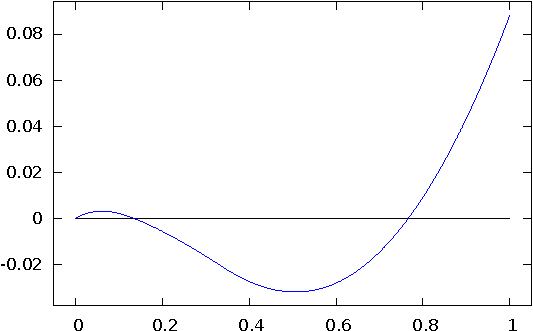
\includegraphics{figures/calculus_derivatives3},
\par\end{center}

\noindent yang akan kita sebut $F$, dapat dengan mudah disangka sebagai
polinom kubik atau polinom berderajat lebih tinggi, padahal fungsi
ini sama sekali tidak sesederhana itu. Pertama, domainnya adalah interval
$[0,1]$, sehingga grafik yang ditampilkan merupakan keseluruhan grafiknya.
Kedua, fungsi ini hanya memiliki dua turunan. Ketiga, definisinya
agak tidak lazim. Kita akan segera membahasnya lebih lanjut.

Di sini kita berhadapan dengan antiturunan dari suatu fungsi interpolasi
fraktal. Fungsi interpolasi adalah fungsi yang grafiknya melalui sekumpulan
titik yang ditentukan. Fungsi ini kebetulan bersifat fraktal, sehingga
merupakan fungsi interpolasi \textit{fraktal}. Fungsi interpolasi
fraktal $f$ melalui
\begin{equation}
(0,.123),\ (.33,-.123),\mbox{ dan }(1,.5)\label{eq:interpolationPoints}
\end{equation}
sedemikian rupa sehingga grafik yang ditampilkan adalah grafik antiturunannya.
Ketidaklaziman definisi $F$ berasal dari ketidaklaziman definisi
$f$:
\[
f(x)=\begin{cases}
f_{1}+c_{1}\frac{x}{\alpha}+d_{1}f\left(\frac{x}{\alpha}\right), & 0\leq x\leq\alpha\\
f_{2}+c_{2}\frac{x-\alpha}{1-\alpha}+d_{2}f\left(\frac{x-\alpha}{1-\alpha}\right), & \alpha\leq x\leq1
\end{cases}
\]
dengan
\[
\begin{gathered}f_{1}=\frac{8979}{100000},\ c_{1}=-\frac{34779}{100000},\ d_{1}=\frac{27}{100}\\
f_{2}=-\frac{75891}{550000},\ c_{2}=\frac{317391}{550000},\ d_{2}=\frac{67}{550}\\
\alpha=\frac{33}{100}.
\end{gathered}
\]

\noindent\begin{digression}{Fungsi Interpolasi Fraktal}

\noindent Fungsi interpolasi fraktal dapat melalui lebih dari tiga
titik. Bahkan, tiga merupakan jumlah minimum titiknya. Secara umum,
untuk $n\geq3$, andaikan $x_{1}<x_{2}<\cdots<x_{n}$. Fungsi interpolasi
fraktal linear (terdapat jenis fungsi interpolasi fraktal lainnya)
yang melalui setiap titik
\[
(x_{1},y_{1}),(x_{2},y_{2}),\ldots,(x_{n},y_{n})
\]
dan berdomain $[x_{1},x_{n}]$ didefinisikan oleh transformasi linear
\[
L_{i}\left(\begin{array}{c}
x\\
y
\end{array}\right)=\left(\begin{array}{cc}
a_{i} & 0\\
c_{i} & d_{i}
\end{array}\right)\left(\begin{array}{c}
x\\
y
\end{array}\right)+\left(\begin{array}{c}
e_{i}\\
f_{i}
\end{array}\right),\quad i=1,2,\ldots,n-1.
\]
Parameter $a_{i}$, $c_{i}$, $e_{i}$, serta $f_{i}$ dihitung berdasarkan
syarat bahwa fungsi tersebut menginterpolasi titik-titik yang diberikan.
Secara khusus, kita mensyaratkan
\[
L_{i}\left(\begin{array}{c}
x_{1}\\
y_{1}
\end{array}\right)=\left(\begin{array}{c}
x_{i}\\
y_{i}
\end{array}\right)\mbox{ dan }L_{i}\left(\begin{array}{c}
x_{n}\\
y_{n}
\end{array}\right)=\left(\begin{array}{c}
x_{i+1}\\
y_{i+1}
\end{array}\right).
\]
Parameter $d_{i}$ adalah parameter bebas dengan pembatasan $|d_{i}|<1$.
Dengan perhitungan aljabar langsung dapat ditunjukkan bahwa
\begin{eqnarray*}
a_{i} & = & \frac{x_{i+1}-x_{i}}{x_{n}-x_{1}}\\
c_{i} & = & \frac{y_{i+1}-y_{i}-d_{i}(y_{n}-y_{1})}{x_{n}-x_{1}}\\
e_{i} & = & x_{i}-a_{i}x_{1}\\
f_{i} & = & y_{i}-c_{i}x_{1}-d_{i}y_{1}.
\end{eqnarray*}

Secara bersama-sama, transformasi $L_{i}$ mendefinisikan fungsi $f$,
dengan setiap $L_{i}$ menangani subselang $[x_{i},x_{i+1}]$ dari
domain tersebut. $L_{i}\left(\begin{array}{c}
x\\
y
\end{array}\right)=\left(\begin{array}{c}
a_{i}x+e_{i}\\
c_{i}x+d_{i}y+f_{i}
\end{array}\right)$, sehingga ketika $L_{i}$ memetakan $x$ ke $a_{i}x+e_{i}$, transformasi
tersebut secara bersamaan memetakan $y$ ke $c_{i}x+d_{i}y+f_{i}$.
Karena $L_{i}$ menerapkan pemetaan ini pada fungsi $f$, harus berlaku
$f(a_{i}x+e_{i})=c_{i}x+d_{i}f(x)+f_{i}$ pada $[x_{1},x_{n}]$, atau
secara ekuivalen,
\[
f(x)=f_{i}+c_{i}\left(\frac{x-e_{i}}{a_{i}}\right)+d_{i}f\left(\frac{x-e_{i}}{a_{i}}\right)\mbox{ pada }[x_{i},x_{i+1}].
\]
Dengan menyatukan seluruh bagian tersebut, $f$ didefinisikan oleh
\[
f(x)=\begin{cases}
h_{1}(x), & x_{1}\leq x\leq x_{2}\\
h_{2}(x), & x_{2}\leq x\leq x_{3}\\
 & \vdots\\
h_{n-1}(x), & x_{n-1}\leq x\leq x_{n}
\end{cases}
\]
dengan
\[
h_{i}(x)=f_{i}+c_{i}\left(\frac{x-e_{i}}{a_{i}}\right)+d_{i}f\left(\frac{x-e_{i}}{a_{i}}\right).
\]
Akibatnya, $F(x)=\int_{x_{1}}^{x}f(t)\,dt$ didefinisikan oleh
\[
F(x)=\begin{cases}
\int_{x_{1}}^{x}h_{1}(t)dt, & x_{1}\leq x\leq x_{2}\\
F(x_{2})+\int_{x_{2}}^{x}h_{2}(t)dt, & x_{2}\leq x\leq x_{3}\\
 & \vdots\\
F(x_{n-1})+\int_{x_{n-1}}^{x}h_{n-1}(t)dt, & x_{n-1}\leq x\leq x_{n}
\end{cases}
\]
tanpa syarat tambahan, sedangkan $f'(x)$ didefinisikan oleh
\[
f'(x)=\begin{cases}
h_{1}'(x), & x_{1}\leq x\leq x_{2}\\
h_{2}'(x), & x_{2}<x\leq x_{3}\\
 & \vdots\\
h_{n-1}'(x), & x_{n-1}<x\leq x_{n}
\end{cases}
\]
asalkan $f'$ ada! Jika $\left|\frac{d_{i}}{a_{i}}\right|<1$ untuk
setiap $i$, maka turunannya ada hampir di mana-mana, tetapi pada
umumnya tidak kontinu. Jika selain itu berlaku $h_{i}'(x_{i+1})=h_{i+1}'(x_{i+1})$
untuk setiap $i=1,2,\ldots,n-2$, maka turunannya ada dan kontinu.
\begin{description}
\item [{Rujukan}] \cite[Bab 6]{barnsley}
\end{description}
\noindent\end{digression}

\noindent Definisi $f$ merujuk pada dirinya sendiri. Nilai-nilainya
didefinisikan, antara lain, melalui nilai-nilai fungsi itu sendiri!
Karena itu, penghitungan nilai fungsi ini agak berbeda dari penghitungan
nilai fungsi biasa. Sebagai contoh, karena $f$ melalui titik-titik
\ref{eq:interpolationPoints}, harus berlaku $f(0)=.123$, $f(.33)=-.123$,
dan $f(1)=.5$, yang dapat kita periksa dengan cukup mudah. Menurut
definisi,
\[
f(0)=f_{1}+d_{1}f(0)=.08979+.27f(0)
\]
 sehingga $f(0)$ didefinisikan sebagian oleh nilainya sendiri. Kita
perlu menyelesaikan persamaan $f(0)=.08979+.27f(0)$ untuk memperoleh
$f(0)$. Dengan demikian, kita memperoleh $f(0)=\frac{.08979}{.73}=.123$,
seperti yang dijanjikan. Sekali lagi menurut definisi, 
\[
f(1)=f_{2}+c_{2}+d_{2}f(1)=-\frac{75891}{550000}+\frac{317391}{550000}+\frac{67}{550}f(1).
\]
Dengan menyelesaikan persamaan tersebut terhadap $f(1)$, kita memperoleh
$f(1)=\frac{-\frac{75891}{550000}+\frac{317391}{550000}}{1-\frac{67}{550}}=\frac{1}{2}$,
seperti yang dijanjikan. Karena $\alpha=.33$, definisi tersebut sebenarnya
memberikan dua cara untuk menghitung $f(.33)$. Menurut bagian pertama
definisi $f$,
\begin{eqnarray*}
f(.33)=f(\alpha) & = & f_{1}+c_{1}+d_{1}f(1)\\
 & = & \frac{8979}{100000}-\frac{34779}{100000}+\frac{27}{100}\cdot\frac{1}{2}\\
 & = & -.123.
\end{eqnarray*}
Sekarang adalah saat yang tepat untuk memverifikasi bahwa $f(\alpha)=-.123$
juga berlaku menurut bagian kedua definisi $f$. Cobalah! Menghitung
nilai-nilai lain dari $f$ mungkin sedikit lebih menantang, tetapi
beberapa di antaranya masih cukup mudah. $\alpha^{2}<\alpha$ dan
$\alpha+(1-\alpha)\alpha>\alpha$, sehingga
\begin{eqnarray*}
f(\alpha^{2}) & = & f_{1}+c_{1}\alpha+d_{1}f\left(\alpha\right)\\
 & = & \frac{8979}{100000}-\frac{34779}{100000}\cdot\frac{33}{100}+\frac{27}{100}\cdot\left(-\frac{123}{1000}\right)\\
 & = & -.0581907\\
f(\alpha+(1-\alpha)\alpha) & = & f_{2}+c_{2}\alpha+d_{2}f\left(\alpha\right)\\
 & = & -\frac{75891}{550000}+\frac{317391}{550000}\cdot\frac{33}{100}+\frac{67}{550}\cdot\left(-\frac{123}{1000}\right)\\
 & = & \frac{2060703}{55000000}\\
 & = & .0374673\overline{27}
\end{eqnarray*}
Dengan tingkat kesulitan yang serupa, sekarang Anda dapat menghitung
\[
\begin{gathered}f(\alpha^{3}),\ f(\alpha(\alpha+(1-\alpha)\alpha)),\ f(\alpha+(1-\alpha)\alpha^{2}),\\
\mbox{dan }f(\alpha+(1-\alpha)(\alpha+(1-\alpha)\alpha)).
\end{gathered}
\]
Jawaban \vpageref{ans:evaluatingf}. Secara lebih umum, setelah Anda
menghitung $f(x)$ untuk suatu nilai $x$, Anda kemudian dapat menghitung
$f(\alpha x)$ dan $f(\alpha+(1-\alpha)x)$ dari nilai tersebut.

Setelah memahami $f$, kita mendefinisikan $F$ dengan $F(x)=\int_{0}^{x}f(t)\,dt$
untuk setiap $x\in[0,1]$. Dengan mengintegralkan $f(x)$, kita memperoleh
\[
F(x)=\begin{cases}
f_{1}x+\frac{c_{1}x^{2}}{2\alpha}+\alpha d_{1}F\left(\frac{x}{\alpha}\right), & 0\leq x\leq\alpha\\
F(\alpha)+f_{2}\left(x-\alpha\right)+\frac{c_{2}\left(x-\alpha\right)^{2}}{2(1-\alpha)}+(1-\alpha)d_{2}F\left(\frac{x-\alpha}{1-\alpha}\right), & \alpha\leq x\leq1
\end{cases}
\]
dengan kedua rumus tersebut sekali lagi berlaku ketika $x=\alpha$.
Sama seperti $f$, fungsi $F$ merujuk pada dirinya sendiri. Untuk
mencari nilai-nilai $F$, kita harus menjalani proses yang sama seperti
ketika mencari nilai-nilai $f$. Sebagai permulaan, $F(0)=\alpha d_{1}F(0)\Rightarrow(1-\alpha d_{1})\cdot F(0)=0,$
tetapi $\alpha$ dan $d_{1}$ keduanya kurang dari 1, sehingga $1-\alpha d_{1}\neq0$.
Oleh karena itu,
\[
F(0)=\frac{0}{1-\alpha d_{1}}=0.
\]
Nilai ini juga dapat kita hitung melalui integrasi: $F(0)=\int_{0}^{0}f(t)\,dt=0$.
Selanjutnya, menurut rumus tersebut,
\[
\begin{gathered}F(1)=F(\alpha)+(1-\alpha)\left(f_{2}+\frac{c_{2}}{2}+d_{2}F(1)\right)\\
\mbox{dan}\\
F(\alpha)=\alpha\left(f_{1}+\frac{c_{1}}{2}+d_{1}F(1)\right),
\end{gathered}
\]
yang merupakan sistem dua persamaan dengan dua peubah yang tidak diketahui,
yaitu $F(\alpha)$ dan $F(1)$. Solusinya adalah
\[
\begin{gathered}F(\alpha)=-\frac{121012947}{6081400000}\approx-.01989886325517151\\
F(1)=\frac{5361861}{60814000}\approx0.0881682014009932.
\end{gathered}
\]
Setelah memperoleh ketiga nilai $F(0),\ F(\alpha),$ dan $F(1)$,
kita dapat menghitung nilai-nilai lainnya seperti sebelumnya. Kedua
nilai $F(\alpha x)$ dan $F(\alpha+(1-\alpha)x)$ sama-sama bergantung
pada nilai $F(x)$. Jadi, kita dapat menghitung $F(\alpha^{2})$ dan
$F(\alpha+(1-\alpha)\alpha)$: 
\begin{eqnarray*}
F(\alpha^{2}) & = & f_{1}\alpha^{2}+\frac{c_{1}\alpha^{3}}{2}+\alpha d_{1}F\left(\alpha\right)\\
 & = & \frac{10678194456039}{6081400000000000}\\
 & \approx & .001755877668964219\\
F(\alpha+(1-\alpha)\alpha) & = & F(\alpha)+f_{2}\left(1-\alpha\right)\alpha+\frac{c_{2}\left(1-\alpha\right)\alpha^{2}}{2}+(1-\alpha)d_{2}F\left(\alpha\right)\\
 & = & -\frac{94196657189979}{3040700000000000}\\
 & \approx & -.03097860926430723.
\end{eqnarray*}
Sekarang Anda dapat menghitung sendiri $F(\alpha^{3})$, $F(\alpha(\alpha+(1-\alpha)\alpha))$,
$F(\alpha+(1-\alpha)\alpha^{2})$, serta $F(\alpha+(1-\alpha)(\alpha+(1-\alpha)\alpha))$.
Jawaban \vpageref{ans:evaluatingF}. Anda tidak perlu bersusah payah
menghitung nilai-nilai ini secara eksak. Hal itu memerlukan sistem
aljabar komputer dengan presisi arbitrer dan bukan merupakan tujuan
sebenarnya. Tujuannya adalah memastikan bahwa Anda memahami cara melakukan
perhitungannya. Gunakan kalkulator atau Octave beserta nilai-nilai
hampiran yang telah dihitung.

\subsection{Turunan $f$ dan grafik lainnya}

Fungsi $f$ memiliki turunan yang kontinu. Bahkan, parameter-parameter
yang mendefinisikan $f$ dipilih secara khusus agar turunannya ada
dan kontinu. Dengan menurunkan $f$, kita memperoleh
\[
f'(x)=\begin{cases}
\frac{c_{1}}{\alpha}+\frac{d_{1}}{\alpha}f'\left(\frac{x}{\alpha}\right), & 0\leq x\leq\alpha\\
\frac{c_{2}}{1-\alpha}+\frac{d_{2}}{1-\alpha}f'\left(\frac{x-\alpha}{1-\alpha}\right), & \alpha\leq x\leq1
\end{cases}
\]
 dan seperti sebelumnya, kita dapat memeriksa bahwa definisi tersebut
konsisten ketika $x=\alpha$:
\[
\begin{gathered}f'(0)=\frac{c_{1}}{\alpha}+\frac{d_{1}}{\alpha}f'(0)\Rightarrow f'(0)=\frac{c_{1}}{\alpha-d_{1}}=-\frac{11593}{2000}=\text{\textminus}5.7965\\
f'(1)=\frac{c_{2}}{1-\alpha}+\frac{d_{2}}{1-\alpha}f'(1)\Rightarrow f'(1)=\frac{c_{2}}{1-\alpha-d_{2}}=\frac{105797}{100500}\approx1.052706467661692\\
f'(\alpha)=\frac{c_{1}}{\alpha}+\frac{d_{1}}{\alpha}f'(1)=-\frac{141949}{737000}\approx-.1926037991858887\\
f'(\alpha)=\frac{c_{2}}{1-\alpha}+\frac{d_{2}}{1-\alpha}f'(0)=-\frac{141949}{737000}\approx-.1926037991858887.
\end{gathered}
\]
Nilai-nilai lain dari $f'$ dapat dihitung dengan cara yang digunakan
untuk $f$ dan $F$. Grafik $f$ dan $f'$ ditampilkan pada Gambar
\ref{fig:Graphf} dan \ref{fig:Graphfprime}. 
\begin{figure}

\caption{\label{fig:Graphf}Grafik $f$.}

\centering{}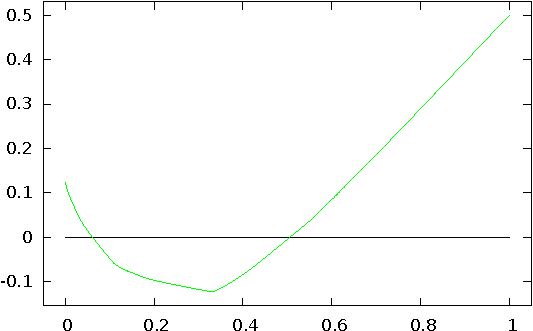
\includegraphics{figures/calculus_derivatives2}
\end{figure}
 
\begin{figure}

\caption{\label{fig:Graphfprime}Grafik $f'$.}

\begin{centering}
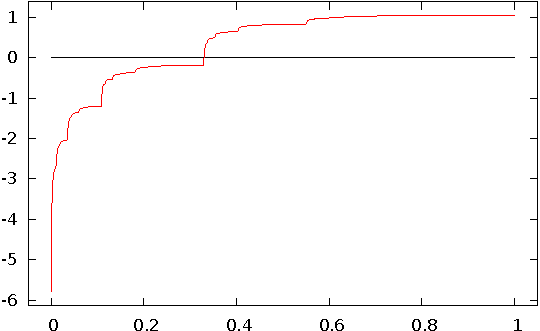
\includegraphics{figures/calculus_derivatives1}
\par\end{centering}
\end{figure}

Demikianlah pembahasannya. Sekarang, cobalah mencari akar ketiga fungsi
tersebut. Kode Octave berikut akan membantu Anda mengevaluasi fungsi-fungsi
itu pada titik mana pun dan sangat menghemat waktu!

\subsection{Octave}

\begin{verbatim}
%%%%%%%%%%%%%%%%%%%%%%%%%%%%%%%%%%%%%%%%%%%%%%%%%%%%%%%%%%
% Written by Dr. Len Brin               19 February 2014 %
% Purpose: Calculate values of the fractal interpolating %
%        function, f, passing through                    %
%        (0,f_0), (alpha,f_alpha), and (1,f_1),          %
%        its derivative and its integral.                %
% INPUT: value at which to evaluate, x; array of values, %
%        f = [f_0,f_alpha,f_1]; alpha; scaling factors   %
%        d1 and d2.                                      %
% OUTPUT: y=f'(x); yy=f(x); yyy=F(x).                    %
%%%%%%%%%%%%%%%%%%%%%%%%%%%%%%%%%%%%%%%%%%%%%%%%%%%%%%%%%%
function [y,yy,yyy] = fractalInterpolator(x,f,alpha,d1,d2)
  f1=f(1)*(1-d1);
  c1=f(2)-d1*f(3)-f1;
  f2=f(2)-d2*f(1);
  c2=(1-d2)*f(3)-f2;
  F1=(alpha*(f1+c1/2)+(1-alpha)*(f2+c2/2))/(1-(1-alpha)*d2-alpha*d1);
  FA=alpha*(f1+c1/2+d1*F1);
  l=0;
  r=1;
  a=[];
  if (alpha>1/2)
    its=floor(log(10^-16)/log(alpha));
  else
    its=floor(log(10^-16)/log(1-alpha));
  end%if
  for i=1:its
    if (alpha>1/2)
      h = (r-l)*alpha;
      m = l+h;
    else
      h = (r-l)*(1-alpha);
      m = r-h;
    end%if
    if (x<m)
      a(i)=0;
      r=m;
    else
      a(i)=1;
      l=m;
    end%if
  end%for
  x=0;
  y=c1/(alpha-d1);
  yy=f(1);
  yyy=0;
  for i=its:-1:1
    if (a(i)==0)
      y=(c1+d1*y)/alpha;
      yy=c1*x+d1*yy+f1;
      yyy=alpha*(f1*x+c1/2*x*x+d1*yyy);
      x=alpha*x;
    else
      y=(c2+d2*y)/(1-alpha);
      yy=c2*x+d2*yy+f2;
      yyy=FA+(1-alpha)*(f2*x+c2/2*x*x+d2*yyy);
      x=alpha+(1-alpha)*x;
    end%if
  end%for
end%function 
\end{verbatim}\texttt{fractalInterpolator.m} dapat diunduh dari \href{http://lqbrin.github.io/tea-time-numerical/ancillaries.html}{situs pendamping}.

\subsection*{Jawaban}
\begin{description}
\item [{Menghitung}] nilai~$f$: \label{ans:evaluatingf}Berikut adalah
beberapa nilai $f$:
\begin{eqnarray*}
f(\alpha^{3}) & \approx & .03620418000000000\\
f(\alpha(\alpha+(1-\alpha)\alpha)) & \approx & -.09176089063636364\\
f(\alpha+(1-\alpha)\alpha^{2}) & \approx & -.08222890363636364\\
f(\alpha+(1-\alpha)(\alpha+(1-\alpha)\alpha)) & \approx & .1846063473223140.
\end{eqnarray*}
\item [{Menghitung}] nilai~$F$: \label{ans:evaluatingF}Berikut adalah
beberapa nilai $F$:
\begin{eqnarray*}
F(\alpha^{3}) & \approx & .002702687013731212\\
F(\alpha(\alpha+(1-\alpha)\alpha)) & \approx & -.003859289400223274\\
F(\alpha+(1-\alpha)\alpha^{2}) & \approx & -.02753062961856850\\
F(\alpha+(1-\alpha)(\alpha+(1-\alpha)\alpha)) & \approx & -.01466250212441314.
\end{eqnarray*}
\end{description}

